%% TODO: finish application to IBM. 2 (and maybe 3 and 4 species). Habitat loss. Single pp-pair from large simulation, and functional grouping.
%%  			> 3 species Jhat not wokring (for chain - ensemble_K estimates are too large. Why? Try other 3sp nets? Other options...)

%% TODO: ODE application to Holling model - quaility versus noise and sampling, and Range sampling (conclude nice concept but very sucetible to noise)

%% TODO:  fill in [REF]S
%% TODO:  sort out noise: check equations(outline.pdf and email to MG dated 12/12/14) & simulations.
%% TODO:  edit FR example figure
%% TODO:  examples section - with inference

%% TODO: be able to derive Timme method on paper - look at matrix calculus notation
%% TODO: conduct local stability analysis for models, and reduce parameter space by subsitution.
%% TODO: include stability analysis in section on simulation procedure?

%% TODO: refer to cite{kefi2012more} if extending this to non-trophic interactions...

\section{Motivation}
\label{sec:motivate_interactions}
% more emphasis on interspecific interactions.
In this chapter we investigate the possibility of quantifying species interaction strengths from observed population dynamics. This was discussed at length in the introduction (section \ref{sec:introduction}), however we now reiterate some of the important points here and to motivate our approach to the problem.

%Inter-specific interactions are one of the major mechanisms that drive ecological processes. For example trophic interactions (e.g. predator-prey) define the pathways along which energy flows through an ecological community [REF], and are responsible for both top-down and bottom-up regulation of species abundances [REF]. Similary mutualistic and competitive interactions play an important role in shaping communities [REF]. However in nature the are many other mechanisms at work, such as seasonality. This, coupled with the difficulty in obtaining high resolution empirical data ahve made it very challenging to quantify the importantce of species interactions in generating observed spatila and temporal patterns in species abundances. 

\begin{itemize}
	\item metrics for interaction strength (choice of IM metric)
	\item hare-lynx dataset (ongoing debate!)
	\item Availability of time-series data. Plankton system (complications! e.g. seasonality)
	\item Motivate simulation approach (known interactions)
	\item Timme approach to fit GLV (use of GLV in general - constant interaction strengths)
	\item Simplify the problem (two species predator prey, but see extension)
\end{itemize}

We implement and test a novel method for quantifying species interactions from population dynamics. Initially we test this method using two distinct ODE simulation models to generate the population dynamics. These two models are referred to as the \emph{linear} and \emph{holling} models. The GLV can fit the \emph{linear} model exactly. Therefore the results presented in section \ref{sec:res_glv} serve as a test of our numerical method. We characterise the robustness of the method to the addition of noise, and under sparsity of sampling. The \emph{holling} model cannot be fitted exactly by the GLV because it uses a different form of \emph{functional response}. Therefore applying our method to population dynamics simulated using the \emph{holling} model provides a test of its ability to give approximate estimates of interaction strength, when underlying structure of the system is not of GLV type. This is also tested in the presence noise and under sparse sampling, and the results are presented in section \ref{sec:res_hii}. In section \ref{sec:res_range_sampling} we provide a preliminary look at how the method could be used to determine the type of functional response present, by observing the dynamics. Having characterised the performance of our method using ODE models, we then apply it, in section \ref{sec:ibm}, to dynamics generated using the IBM model of previous chapters. This represents a first step towards applying the method to empirical data, since it involves a spatial system and a larger number of species. We conclude the chapter with a discussion of how the method could be developed further towards empirical application. 

%To mention in this section:
%\begin{itemize}
%	\item IM metric: 'key to this chapter' (discuss other metrics, Berlow et al.)
%
%	\item hare-lynx dataset (ODE models not fit, other explainations, quality of data)
%	\item IBM models 
%	\item ODE population models and FR (importance of FR in defining interactions)
%	\item interaction networks, species roles and plankton
%	\item how strong are interactions? (quantitative networks)
%
%	\item Lacking suitable data - for which time-series and interaction (strengths) known..
%	\item Focus on PP interactions..but importance of others and extension possible
%\end{itemize}

% All inter-specific interactions play a role in generating the temporal pattern of species abundances that we call \emph{population dynamics}. A well known example of this is the phenomenon of predator-prey oscialltions, which are thought to have been exhibited by hare and lynx populations in Hudson Bay, Cananda [REF]. Predator-prey oscillations will play an important role in this chapter.


%The general goal is to quantify inter-specific interaction strengths from observed population dynamics. As discussed, we currenlty lack suitable empircal data to do this (section \ref{sec:motivate_interactions}). Therefore we develop a methodolgy using \emph{simulated} population dynamcis. In the future this method could be applied to empircal abudnance time-series (see discussion in section \ref{sec:discussion}). The population models used for simulation are, for the most part, standard ordinary differential equation (ODE) models. These are outlined in section \ref{sec:models}. However we also present a preliminary application of our methdology to dynamics generated using the individual-based model from the previous chapters (section \ref{sec:ibm}). To quantify the interaction strengths between species from their simulated dynamics we adapt a method from \cite{shandilya2011inferring}. In short the method is used to fit a generalised Lotka-Volterra (GLV) model to the dynamics, giving numerical estimates of the interaction terms. The method is detailed in section \ref{sec:timme} and the use of the GLV model to quantify interaction strengths is justified in section \ref{sec:interaction_strength}. %% more on interaction strenght and GLV model here?


%We test a numerical method for estimating species interaction strengths from population dynamics. The method, described in section \ref{sec:timme}, works by fitting a generalised Lotka-Volterra model (GLV) to discrete observations of the dynamics. Therefore we obtain estimates of the `best fit' GLV parameters, given the observed dynamics. These parameters include intrinsic growth rate coefficients for each species, and constant coefficients defining the strength of coupling between all species in the system (see section \ref{sec:interaction_strength}).

%We test the method on two species predator-prey dynamics, which are simulated using ODE models. A general framework for the ODE modelling is given in section \ref{sec:models}, from which we derive two distinct models. 

%% some of this??
%To simulate population dynamics we use coupled ordinary differential equation (ODE) models. Although we focus on dynamics generated by predator-prey interactions, the ODE modelling framework may be adapted to model other types of interaction (e.g. mutulaism, competition). ODE models have been used extensively to simulate predator-prey dynamics at the species level [REFS]. They have several limitations in their usefullness. which are discussed in \ref{sec:discussion}. However they are a suitable choice for us becuse the equations explictly contain a term that defines the interactions between species. Therefore we are able to simulate populations dynamics for which we know the analytic form of all inter-specific interactions involved. This is the key to being able to test our method for quantifying interaction strengths [SECTION?].   


\section{Methodology}
\label{sec:methods}

%% reorder and state where IM is given for simulation..

\begin{figure}[h]
\centering 
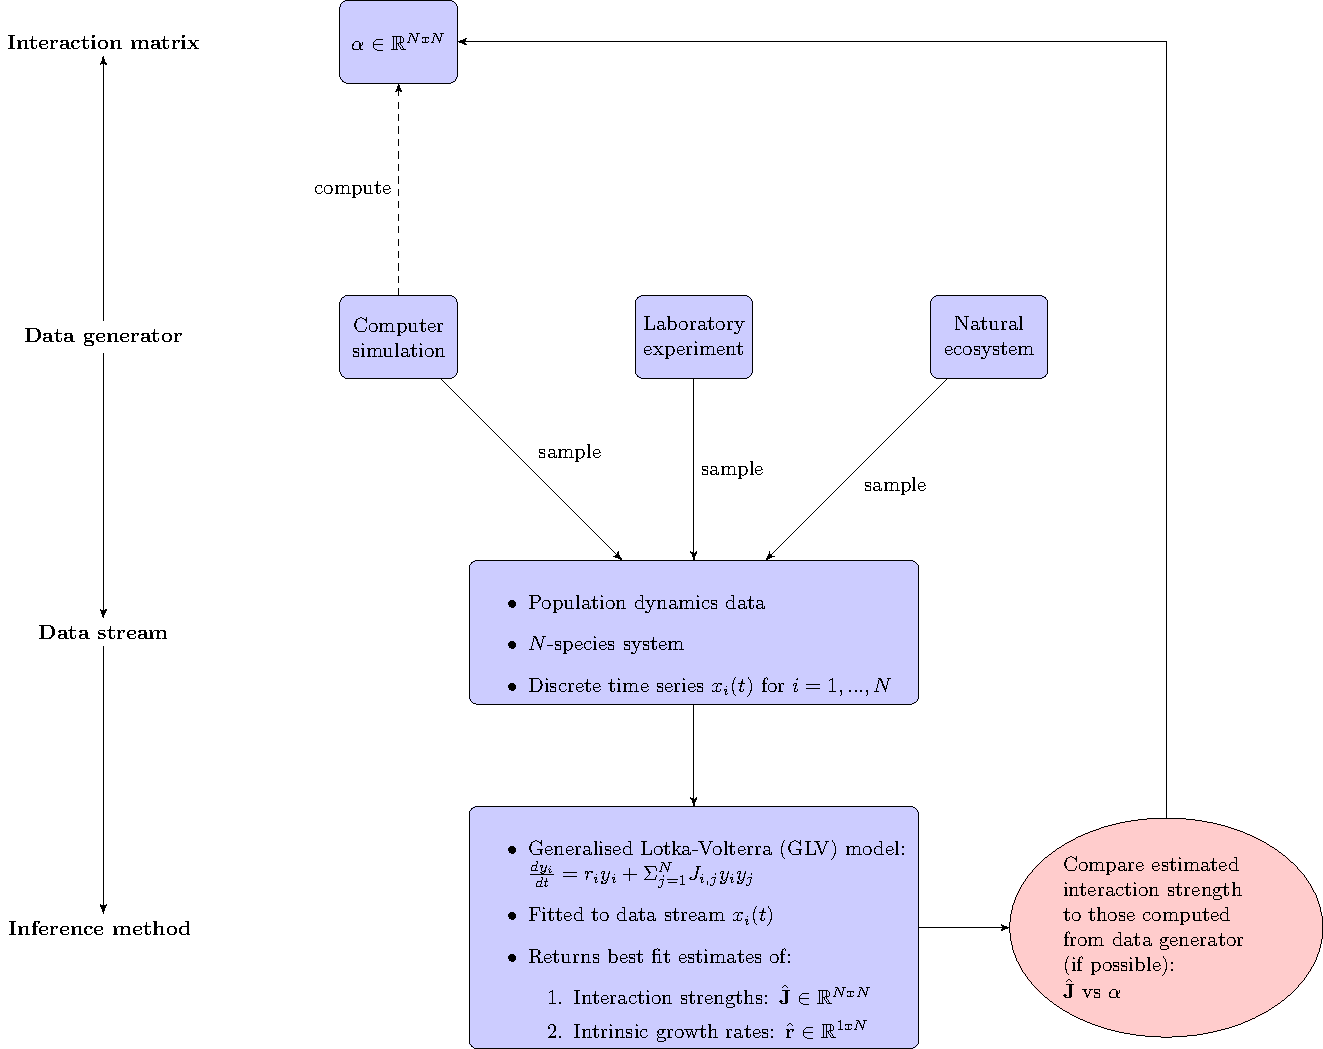
\includegraphics[width=\textwidth]{{{flow_chart/flow_chart}}}
\caption{This is what we do.} 
\label{fig:method_flow}
\end{figure}


To summarise our methodology, we simulate population dynamics then sample these dynamics and fit a \emph{generalised Lotka-Volterra} (GLV) model. The fitted GLV parameters give us estimates of the species interaction strengths (and other parameters), which we then compare to those used in the original simulation. The details of all the stages are given below. In section \ref{sec:interaction_strength} the \emph{interaction matrix} (IM) is introduced. The IM is the metric used to quantify the strength of species interactions and is key to this chapter. We also introduce the \emph{generalised Lotka-Volterra} (GLV) model, and show that this model has constant interaction strengths, given by the coupling matrix $J$. In section \ref{sec:models} we give a general framework for ODE predator-prey modelling, and derive the two models that we use to simulate population dynamics. We then discuss, in section \ref{sec:simulation_method} the details of how these models are simulated \emph{in silico}, including the selection of model parameters. Section \ref{sec:timme} gives the details of the numerical method we use for fitting the GLV model to sampled population dynamics. In section \ref{sec:method_examples} we give an example of the full methodology in action.

\subsection{Interaction strength}
\label{sec:interaction_strength}

% emphasise that we know the interaction strength for our simulation model

The metric used for species interaction strength is key to this chapter. As discussed in section \ref{sec:motivate_interactions} there are several metrics available [REF]. However there is one that is a natural choice, given our methodology. This metric allows us to calculate the interaction strengths from our simulation models, and to directly compare them to the estimates obtained by fitting the GLV model. The metric is called the \emph{interaction matrix} (IM). The elements of the IM, $\alpha_{ij}$, quantify the effect of a small change in the population density of species $j$ on the per capita growth rate of species $i$ [REF]. Therefore the IM elements are given by:

\begin{equation}
\alpha_{ij} = \frac{\partial}{\partial x_{j}}\left(\frac{1}{x_{i}} \frac{dx_i}{dt} \right),
\label{eq:IM}
\end{equation}

where $x_i$ and $x_j$ are the population densities of species $i$ and $j$ respectively.  In the case of our two species systems the IM is a $2 \times 2$ matrix, but trivially extends to quantify all $N^2$ pair-wise interactions between species in a $N$-species system (including self-interactions). 

Using the IM we are able to calculate the interaction strengths exactly from the models that we use for simulation. This is because they are ODE models with explicit expressions for $dx_i / dt$, so we can evaluate the partial derivative in equation \ref{eq:IM} to obtain analytic forms for all the IM elements ($\alpha_{00}$, $\alpha_{01}$, $\alpha_{10}$,$\alpha_{11}$). Depending on the model used the IM elements are either constants, or are functions of prey density. The interaction strengths for our simulation models are given at the end of section \ref{sec:models}, and are illustrated in figure \ref{fig:fr_example}.

\paragraph*{Generalised Lotka-Volterra.} The GLV model is the extension of the Lotka-Volterra equations to $N$ species. We use this model to fit to simulated population dynamics and obtain estimates of the underlying interaction strengths. The GLV model is given by:

\begin{equation}
\frac{dx_i}{dt} = r_ix_i + \Sigma_{j=1}^N J_{ij}x_ix_j,
\label{eq:glv}
\end{equation}

where $x_i$ is the population density of species $i$; $r_i$ is the intrinsic growth rate; $N$ is the number of species and $J_{ij}$ is the coupling between species $i$ and $j$. Applying equation \ref{eq:IM} to equation \ref{eq:glv} we see that $\alpha_{ij} = J_{ij}$, such that the IM for the GLV model is equal to the coupling matrix. Therefore, by fitting the GLV model to population dynamics, the fitted parameters $J_{ij}$ give us numeric estimates of interaction strength. To perform the fit we use the method detailed in section \ref{sec:timme}.

\subsection{Population models}
\label{sec:models}
%LINEAR IS SAME AS GLV!!
%% Parameter choices. Euler method. Timestep. Extinction boundary contiditions.
%% Conventional to use N,P for predator prey, however our terminology allows easy extension to larger systems..(refer forwards to this)
%% re-order this - good choice first!


We use ordinary differential equation (ODE) models to simulate two species predator-prey dynamics. Therefore the mathematics presented in this section focuses on this case. However the framework may be easily extended to include other interaction types (completion and mutualism), and to model larger systems in a similar way. For a two species system the dynamics are governed by two coupled equations, one for each species. Importantly it is possible, using the IM introduced in section \ref{sec:interaction_strength}, to calculate the species interaction strengths from the model. The model equations take the general form:

\begin{eqnarray}
\frac{dx_0}{dt} &=& G_{0}(x_0) + a_{01}x_1H(x_0,x_1),  \nonumber \\
\frac{dx_1}{dt} &=& G_{1}(x_1) + a_{10}x_1H(x_0,x_1)
\label{eq:two_species}
\end{eqnarray}

where species $x_0$ and $x_1$ are the population densities of the prey and the predator species respectively; the $G_i(x_i)$ are the intrinsic growth functions of each species; the $a_{ij}$ are constant coefficients and $H(x_0,x_1)$ is the functional response (FR) of the predator. This form is standard in the literature [REFS] and many models may be expressed in this way by choosing different functional forms for $G$ and $H$. The coefficients $a_{01}$ and $a_{10}$ are negative and positive respectively, such that the prey losses biomass, and the predator gains biomass as a result of the interaction. These coefficients may be used to introduce asymmetry into the interaction terms. For example it is common to choose $|a_{01}| > |a_{10}|$, to model the inefficiency of the predator in the conversion of biomass from the prey. For the intrinsic growth functions we use the functional forms:  

\begin{eqnarray}
G_0(x_0) &=& r_0x_0\left(1-\frac{x_0}{K_c}\right)  \\
G_1(x_1) &=& -r_1x_1,
\label{eq:two_species}
\end{eqnarray}

where $r_i \in \mathbb{R}^+$ is the intrinsic growth rate of species $i$, and $K_c$ is the carrying capacity of the prey species. Therefore the predator has an exponential intrinsic mortality, whereas the prey species has logistic intrinsic growth. These use of these functional forms in predator-prey modelling was made popular by Rosenzweig and MacArthur [REF]. They are now widely used [REFS]. 

The FR defines the per-predator rate of consumption of prey. We focus on the forms proposed by Holling in the 1950s [REFs], which are also widely used [REFS]. However it is worth noting that various other forms have been proposed and there is an ongoing debate about which to use [REFS] (see discussion in section \ref{sec:discussion}). There are three types of Holling FR, referred to as types I, II, and III. These can be expressed as:

\begin{eqnarray}
H_I(x_0,x_1) &=& x_0,  \label{eq:h1} \\
H_{II}(x_0,x_1) &=& \frac{x_0}{x_0 + K_s},  \label{eq:h2} \\
H_{III}(x_0,x_1) &=& \frac{x_0^2}{x_0^2 + K_s^2},
\end{eqnarray}


where $x_0$ is the prey density, and $K_s$ is the saturation constant for the predator, giving the prey density at which the per-predator consumption rate reaches half-maximum. We choose to narrow our investigation by focusing here on the first two forms: Holling type I and type II. Therefore we have two distinct simulation models, which we refer to as the \emph{linear} and \emph{holling} models.

\paragraph*{Linear model.} 
This model uses the type I FR. As is clear from equation \ref{eq:h1}, type I is the simplest of the Holling functions: the per-predator predation rate increases linearly as the abundance of available prey increases. The slope of this linear relationship given by the $a_{ij}$ parameters in equations \ref{eq:two_species}. The linear FR is the same as is used in the famous Lotka-Volterra equations [REF], meaning that our linear model may be expressed in GLV form (equation \ref{eq:glv}). We may rescale the equations of the linear model in order to reduce the number of parameters. This makes the local stability analysis simpler, and reduces the dimension of the search space when probing the equations numerically via simulation. The re-scaled equations are given by:

\begin{eqnarray}
\frac{d\chi_{0}}{dt} &=& A\chi_0(1-\chi_0) - B\chi_0\chi_1 \label{eq:lin_mod1} \\
\frac{d\chi_{1}}{dt} &=& -\chi_1 + C\chi_0\chi_1 \label{eq:lin_mod2}, 
\end{eqnarray}

where $\chi_0$ and $\chi_1$ are the re-scaled prey and predator population densities respectively; the parameters $A,B,C \in \mathbb{R}^+$. The equilibrium population densities are given by:

\begin{eqnarray}
\chi_{0}^{*} &=& \frac{1}{C} \label{eq:lin_mod_sp1} \\
\chi_{1}^{*} &=& \frac{A}{B}\left(1 - \frac{1}{C}\right) \label{eq:lin_mod_sp2}, 
\end{eqnarray}

Therefore $\chi_{0}^{*}$ is always positive, and $\chi_{1}^{*}$ is positive if $c > 0$. This is a requirement for physical realism, since it is not possible to have negative populations of species. In most applications it is also required that this equilibrium is stable, to allow for the coexistence of species. We use these conditions on the equilibrium for parameter selection, which is discussed in section \ref{sec:simulation_method}. By applying equation \ref{eq:IM} to equations \ref{eq:lin_mod1} and \ref{eq:lin_mod2} we can evaluate the elements of the IM for the linear model. This gives:

\begin{equation}
\alpha_{linear} = 
\begin{bmatrix}
-A & -B \\ C & 0
\end{bmatrix}  	,
\end{equation}

such that all the interaction strengths are constants, which is illustrated in figure \ref{fig:ex_dynamics_linear}.

\paragraph*{Holling model.} 
This model uses the type II FR, which is a non-linear function of prey density. As we can see from equation \ref{eq:h2} and figure \ref{fig:fr_example}, this FR models predator saturation - individuals take a certain amount of time to process and digest prey - such that the response curve flattens out at high prey densities. The difference between the type I and II functions is illustrated in figure \ref{fig:fr_example}. We may perform a similar rescaling as we did with the linear model to reduce the number of parameters. The resulting equations for the holling model are given by:

\begin{eqnarray}
\frac{d\chi_{0}}{dt} &=& A\chi_0(1-\chi_0) - \frac{B\chi_0\chi_1}{\chi_0 + D} \label{eq:hol_mod1} \\
\frac{d\chi_{1}}{dt} &=& -\chi_1 + \frac{C\chi_0\chi_1}{\chi_0 + D} \label{eq:hol_mod2}, 
\end{eqnarray}

where the saturation constant $D \in \mathbb{R}^+$, and the other symbols are the same as in equations \ref{eq:lin_mod1} and \ref{eq:lin_mod2}. The equilibrium populations for this model are given by:

\begin{eqnarray}
\chi_{0}^{*} &=& \frac{D}{C-1} \label{eq:hol_mod_sp1} \\
\chi_{1}^{*} &=& \frac{ACD(C-1-D)}{B(C-1)^2} \label{eq:hol_mod_sp2}, 
\end{eqnarray}

Therefore $\chi_{0}^{*}$ is positive if $C > 1$, $\chi_{1}^{*}$ is positive if $C - D > 1$. Again we use these conditions, and the requirement of stability, to constrain our choice of parameters (\ref{sec:simulation_method}). As we did for the linear model, we can evaluate the IM for the holling model, giving:

\begin{equation}
\alpha_{holling} = 
\begin{bmatrix}
-A + \frac{B\chi_1}{(\chi_0 + D)^2} & \frac{-B}{\chi_0 + D} \\ \frac{CD}{(\chi_0 + D)^2} & 0
\end{bmatrix}  	,
\end{equation}

such that the three non-zero elements of the IM are functions of prey density $\chi_0$, instead of constants. The shape of these interaction functions is shown in figure \ref{fig:fr_example}, and we will return to them in section \ref{sec:method_examples}.


\begin{figure}[h]
\centering 
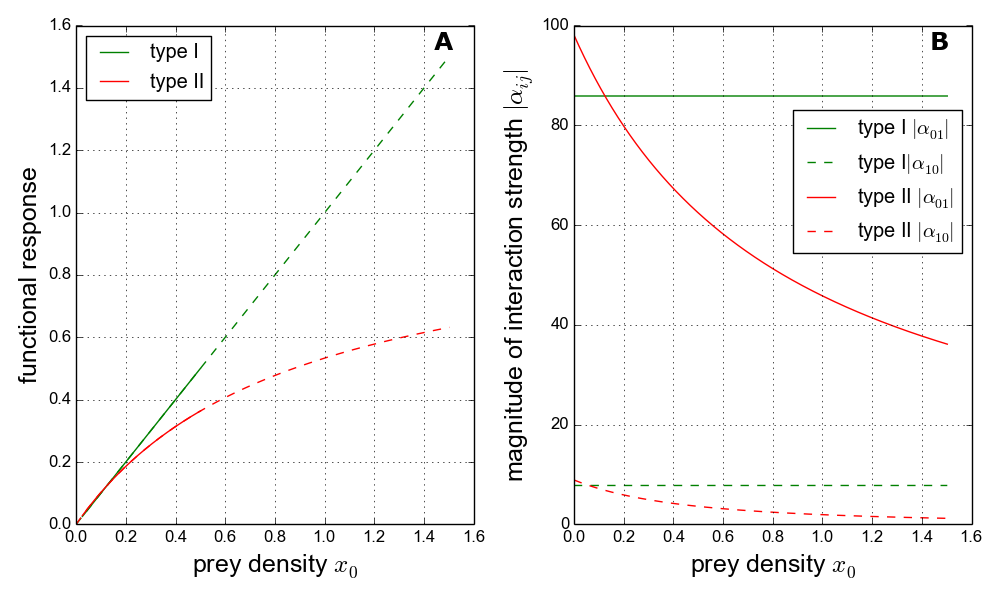
\includegraphics[width=0.8\textwidth]{{{figures/FR_example}}}
\caption{Example of (A) the functional response curve, and (B) the corresponding inter-specific interaction strengths for one parameter set of the \emph{linear} model, and one of the \emph{holling} model.} 
\label{fig:fr_example}
\end{figure}


\subsection{Simulation procedure}
\label{sec:simulation_method}

\begin{center}
\begin{table}
\centering
    \begin{tabular}{| l | l | l | l | l |}

    \hline
     & A & B & C & D\\ \hline
    linear & 0.1 - 100 & 0.1 - 100 & 1 - 100 & N/A \\ \hline
    holling & 0.1 - 100 & 0.1 - 100 & 1.1 - 100 & 0.1-99 \\
    \hline
    \end{tabular}
\caption{Ranges from which parameters were selected unifomrly at random for the two ODE simulation models. The parameters are all allowed to vary over at least three orders of magnitude, to ensure that our investigation covers a large region of parameter space. The restrictions on parameters C and D ensure that it is always possible to acheive an equilibirum population of both species that is strictly positive (see equations \ref{eq:lin_mod_sp1}, \ref{eq:lin_mod_sp2}, \ref{eq:hol_mod_sp1}, \ref{eq:hol_mod_sp2})}
\label{table:p_range}    
\end{table}
\end{center}


%% note we are noew referring to linear and holling simulation models..
We apply a strict recipe when running simulations in order to ensure consistency and to allow comparison of our numerical results. Key to this is the control of certain variables across simulations, and also our method for parameter selection, both of which are discussed below. All simulations are run using the first-order forward Euler approximation to the ODE model. We use additive Gaussian noise to simulate \emph{process error}. Therefore we implement the stochastic difference equation :

\begin{equation}
\label{eq:stochastic_diff}
\chi_{i, t+1} = \chi_{i, t} + \Delta t\Delta\chi_{i,t} + \xi_{i,t},
\end{equation}

where $\Delta t$ is the integration time step, $\Delta\chi_{i}$ is given by the right hand side of ODE model being simulated (e.g. equations \ref{eq:lin_mod1}, \ref{eq:lin_mod2} for the linear model); and the additive noise term $\xi_{i,t} \backsim \mathbb{N}(0, \sigma_{noise}\chi_{i,t}\Delta t)$. The value of $\sigma_{noise}$ is quoted as \emph{noise intensity} in what follows. In the event of stochastic extinction of either species, both population densities are reset to their initial conditions. The case where $\sigma_{noise} = 0$ is referred to as the \emph{deterministic} model. In all the results presented the simulations were run with a time step $\Delta t = 10^{-4}$. All code was implemented in the language \emph{Python}, and large computations were performed on the UoB HPC cluster \emph{Blue Crystal} [REF].

The goal of fitting the GLV model to simulated population dynamics requires that the dynamics contain enough information to perform the fit - it is not possible to fit the a model if species populations are sitting at equilibrium. Therefore we follow the precedent set in [REF], such that all simulated dynamics of the \emph{deterministic models} exhibit two `large amplitude ' oscillations about a stable equilibrium (see condition 2 below). Every simulation is run with the initial population densities set to half of their equilibrium value. This ensures that all systems start consistently away from equilibrium.

\paragraph*{Parameter selection.} We select an ensemble of 100 parameter sets for both simulation models (\emph{linear} and \emph{holling}). Parameters are selected uniformly at random from predefined ranges, which are given in table \ref{table:p_range}. This range ensures that a positive equilibrium population is possible (see equations \ref{eq:lin_mod_sp1}, \ref{eq:lin_mod_sp2}, \ref{eq:hol_mod_sp1}, \ref{eq:hol_mod_sp2}), but also allows for parameters to vary over at least three orders of magnitude so that our investigation covers a large region of parameter space. The selected parameters are then accepted if they meet the following conditions:

\begin{enumerate}
	\item The equilibrium population is positive, and is locally a stable spiral (eigenvalues of the Jacobian have negative real part and complex conjugate imaginary part).
	\item The deterministic dynamics exhibit at least two full rotations in the phase plane before relaxing to within $5\%$ of the equilibrium (Euclidean distance in the phase plane).
	\item The population densities do not differ by more than an order of magnitude, in the deterministic case.
\end{enumerate}

The two parameter sets generated by the above procedure are used for the simulation results presented in section \ref{sec:results}. All simulations , including those with $\sigma_{noise} \neq 0$, are run for the length of time $T_{2P}$ required to achieve two full oscillations in the deterministic case, for that parameter set.

\subsection{Numerical estimation method}
\label{sec:timme}

%% Dealing with extinctions. Range sampling - diagrams!!
%% make use of GLV more explicit

To estimate the inter-specific interaction strengths we use a numerical method, adapted from \cite{shandilya2011inferring}, to fit the GLV model to the population dynamics. The method gives `best fit' estimates of the GLV parameters, which include constant coefficients for the interaction strengths as we saw in section \ref{sec:interaction_strength}. We include here a derivation of the method, slightly adapted and simplified for our purposes. Say the dynamics of the population density of a species $x_i$ is governed by coupled differential equations of the form:

\begin{equation}\label{eq:timme1}
 \dot{x_i} = r_if_i(x_i) + \Sigma_{j=1}^{N}J_{i,j}g_{ij}(x_i,x_j),\\
\end{equation}

where $\dot{x_i} = \frac{d}{dt}x_{i}$; $N$ is the number of species in the system and $i,j$ index the species. The $r_i, J_{ij} \in \mathbb{R}^+$ are constants, and the functions $f_i$ and $g_{ij}$ are known. This form looks familiar, indeed all of the ODE models discussed so far may be expressed in this form - there is an intrinsic growth term, and a linear sum of interaction terms. To express the GLV model (equation \ref{eq:glv}) in this form, we have:

\begin{eqnarray}
f_i(x_i) &=& x_i \\
g_{ij}(x_i,x_j) &=& x_ix_j, 
\end{eqnarray}

It would be possible to use this method to fit models other than the GLV, so long as the functions $f_i$ and $g_{ij}$ are \emph{known and parametrised}. Since the functions $f_i$ and $g_{ij}$ are known there are $N+1$ unknowns in equation \ref{eq:timme1}: $r_i$ and $J_{i,j}$ for $j=1,...,N$. Therefore, if we knew the exact values of $\dot{x_i},x_i$ and the $x_j$'s, at $N+1$ time points, then we could solve the equation for $r_i$ and the $J_{i,j}$'s. However in any practical application our knowledge of the system is not \emph{exact}; the system is subject to noise; and the model may be an imperfect description of the dynamics. So the equation cannot be solved exactly. We must look for an approximate solution. To do this the full state of the system is sampled at $M+1$ time points $t_m$ for $m \in {1,..,M,M+1}$. These samples are used to construct estimates for the states $x_i$ and their time-derivatives $\dot{x}_i$ at $M$ intermediate time points, for every species $i$.

The simplest way to estimate the time-derivatives is to take the finite difference between observations at two consecutive time points, giving estimates:

\begin{equation}\label{eq:timme2}
\hat{\dot{x}}_{i}(\tau_m) := \frac{x_i(t_m) - x_i(t_{m-1})}{t_m - t_{m-1}},\\
\end{equation}

where $\tau_m \in{\mathbb{R}}, m \in{\{1,...,M\}}$ is the midpoint of the two time-points:

\begin{equation}\label{eq:timme3}
\tau_m := \frac{t_{m-1} + t_{m}}{2}.\\
\end{equation}

To evaluate the functions $f_i, g_{ij}$ at these new time-points we must estimate the states $x_i(\tau_m)$ from our observations. We use the linear interpolation:

\begin{equation}\label{eq:timme4}
\hat{x}_{i}(\tau_m) := \frac{x_i(t_{m-1}) + x_i(t_{m})}{2}.\\
\end{equation}

So from equation \ref{eq:timme1} we can now construct $M$ equations using our $M+1$ samples:

\begin{equation}\label{eq:timme5}
\hat{\dot{x}}_{i}(\tau_m) = r_if_{i}(\hat{x}_i(\tau_m)) + \Sigma_{j=1}^{N}J_{i,j}g_{ij}(\hat{x}_i(\tau_m), \hat{x}_j(\tau_m)).\\
\end{equation}

We now simplify the notation such that equation \ref{eq:timme5} may be written 

\begin{equation}\label{eq:timme6}
\hat{\dot{x}}_{i,m} = r_if_{i,m} + \Sigma_{j=1}^{N}J_{i,j}g_{ij,m},\\
\end{equation}

where the subscripts  $i,j$ indicate the species, and $m$ indicates the time-point $\tau_m$ for which the equation holds. This system of $M$ equations can be expressed in matrix form:

\begin{equation}\label{eq:timme7}
X_{i} = J_iG_i,\\
\end{equation}

where we have

\begin{equation}\label{eq:timme8}
X_{i} = 
\begin{pmatrix}
  \hat{\dot{x}}_{i,1} & \hat{\dot{x}}_{i,2} & \cdots & \hat{\dot{x}}_{i,M}
\end{pmatrix}\\
\in{\mathbb{R}^{1 \times M}},
\end{equation}

\begin{equation}\label{eq:timme9}
J_{i} = 
\begin{pmatrix}
  r_i & J_{i,1} & J_{i,2} & \cdots & J_{i,N}
\end{pmatrix}\\
\in{\mathbb{R}^{1 \times(N+1)}},
\end{equation}

\begin{equation}\label{eq:timme10}
G_{i} = 
\begin{pmatrix}
  f_{i,1}  &    f_{i,2} & \cdots & f_{i,M}         \\
  g_{i,1,1} & g_{i,1,2} & \cdots & g_{i,1,M} \\
  g_{i,2,1} & g_{i,2,2} & \cdots & g_{i,2,M} \\
  \vdots    & \vdots    & \ddots & \vdots    \\
  g_{i,N,1} & g_{i,N,2} & \cdots & g_{i,N,M} \\
\end{pmatrix}\\
\in{\mathbb{R}^{(N+1)\times M}}.
\end{equation}

%Here $J_i$ is the $i$th row of the full coupling matrix $J$ and represents the input coupling strengths to the unit $i$. 

The system \ref{eq:timme7} has $N+1$ unknowns ($J_{i,k}$ for $k=1,..,N+1$) and $M$ equations. In the case when $M>N+1$ the system is over constrained and there is no exact solution in general. We look for an approximate solution $\hat{J}_i$ that minimises the error between the LHS and RHS of equation \ref{eq:timme7}. We take the error function:

\begin{equation}\label{eq:timme11}
E_i(\hat{J}_i) = \Sigma_{m=1}^{M}(X_{i,m} - \Sigma_{k=1}^{N+1}\hat{J}_{i,k}G_{i,k,m})^2,
\end{equation}

which we want to minimise with respect to the matrix elements $\hat{J}_{i,k}$. That is

\begin{equation}\label{eq:timme12}
\frac{\partial}{\partial \hat{J}_{i,k}} E_i(\hat{J}_i) \mbeq 0.
\end{equation}

By taking the derivative of the RHS of equation\ref{eq:timme11} we have that:


\begin{eqnarray}
\frac{\partial}{\partial \hat{J}_{i,k'}} E_i(\hat{J}_i) &=& \frac{\partial}{\partial \hat{J}_{i,k'}} [\Sigma_{m=1}^{M}(X_{i,m} - \Sigma_{k=1}^{N}\hat{J}_{i,k}G_{i,k,m})^2] \nonumber \\
    &=& -2\Sigma_{m=1}^{M}[(X_{i,m} - \Sigma_{k=1}^{N}\hat{J}_{i,k}G_{i,k,m})G_{i,k',m}] \nonumber
\end{eqnarray}

To find the minimum of the error function we equate this to zero, giving:

\begin{eqnarray}
0 &=& \Sigma_{m=1}^{M}(-X_{i,m}G_{i,k',m} + G_{i,k',m}\Sigma_{k=1}^{N}\hat{J}_{i,k}G_{i,k,m}) \nonumber \\
  &=& (-X_iG_i^T)_{k'} + \Sigma_{m=1}^{M}G_{i,k',m}(\hat{J}_iG_i)_m   \nonumber \\
  &=& (-X_iG_i^T)_{k'} + \Sigma_{m=1}^{M}(\hat{J}_iG_i)_mG_{i,m,k'}^T  \nonumber \\
   &=& -X_iG_i^T + \hat{J}_iG_iG_i^T 
\end{eqnarray}

Therefore we conclude that:

\begin{equation}\label{eq:timme_a2}
\hat{J}_i = XG^T_i(G_iG^T_i)^{-1},
\end{equation}

which, in our case, is the analytic form for the best estimate of the row corresponding to species $i$ in parameter matrix of the GLV model. For a two species system, by applying equation \ref{eq:timme_a2} to each species, we can obtain the full set of GLV parameter estimates: 

\begin{equation}\label{eq:timme_estimates}
\hat{J} =
\begin{pmatrix}
 \hat{J}_{0,0} & \hat{J}_{0,1} \\
 \hat{J}_{1,0} & \hat{J}_{1,1}
 \end{pmatrix}\\,
\end{equation}

and

\begin{equation}\label{eq:timme_estimates2}
\hat{r} =
\begin{pmatrix}
 \hat{r}_{0} & \hat{r}_{1} 
 \end{pmatrix}\\.
\end{equation}

We perform the computation by constructing the matrices $X_i$ and $G_i$ for both species, and do the matrix multiplication using the \emph{Python} package \emph{numpy}[REF]. The fact that the error minimisation has an analytic solution makes it very computationally efficient, allowing us to perform many replicate calculations. However the performance of the method may be lower than other, more computationally expensive, model fitting algorithms (see discussion section \ref{sec:discussion}). It is possible to assess the goodness of fit achieved by evaluating the error function (equation \ref{eq:timme11}). 

\subsection{Examples}
\label{sec:method_examples}

%% include here an example of both Linear and HII dynamics (with mean interaction strength), and to demonstrate noise levels. And the results that we get from tinference. And an examples of range samplig (refer forwards to dsicusssion) 
Here we show examples of the dynamics of both models, both with and without noise..For the holling model we also show the variability in interaction strengths during the simulations..We also present a table with the results of the GLV, comparing them to the simulation interaction strengths..


\begin{figure}[h]
\centering 
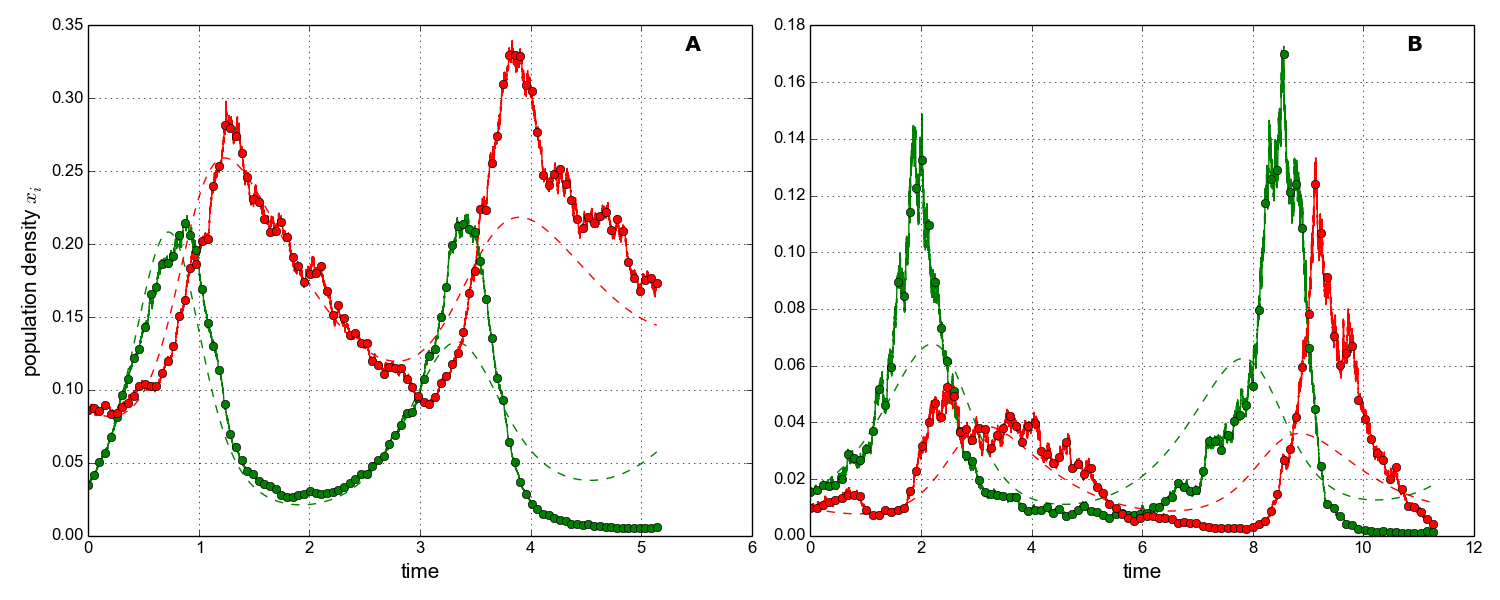
\includegraphics[width=\textwidth]{{{figures/example_dynamics_pID_0_and_87_noise_20.000000}}}
\caption{Example linear dynamics. 100 sampels. Two different parameter sets. A: noise=20. B:noise=50.} 
\label{fig:ex_dynamics_linear}
\end{figure}

\clearpage
%\afterpage{%
\thispagestyle{empty}
\begin{sidewaysfigure}

		\centering      
		\hspace{-3cm}

        %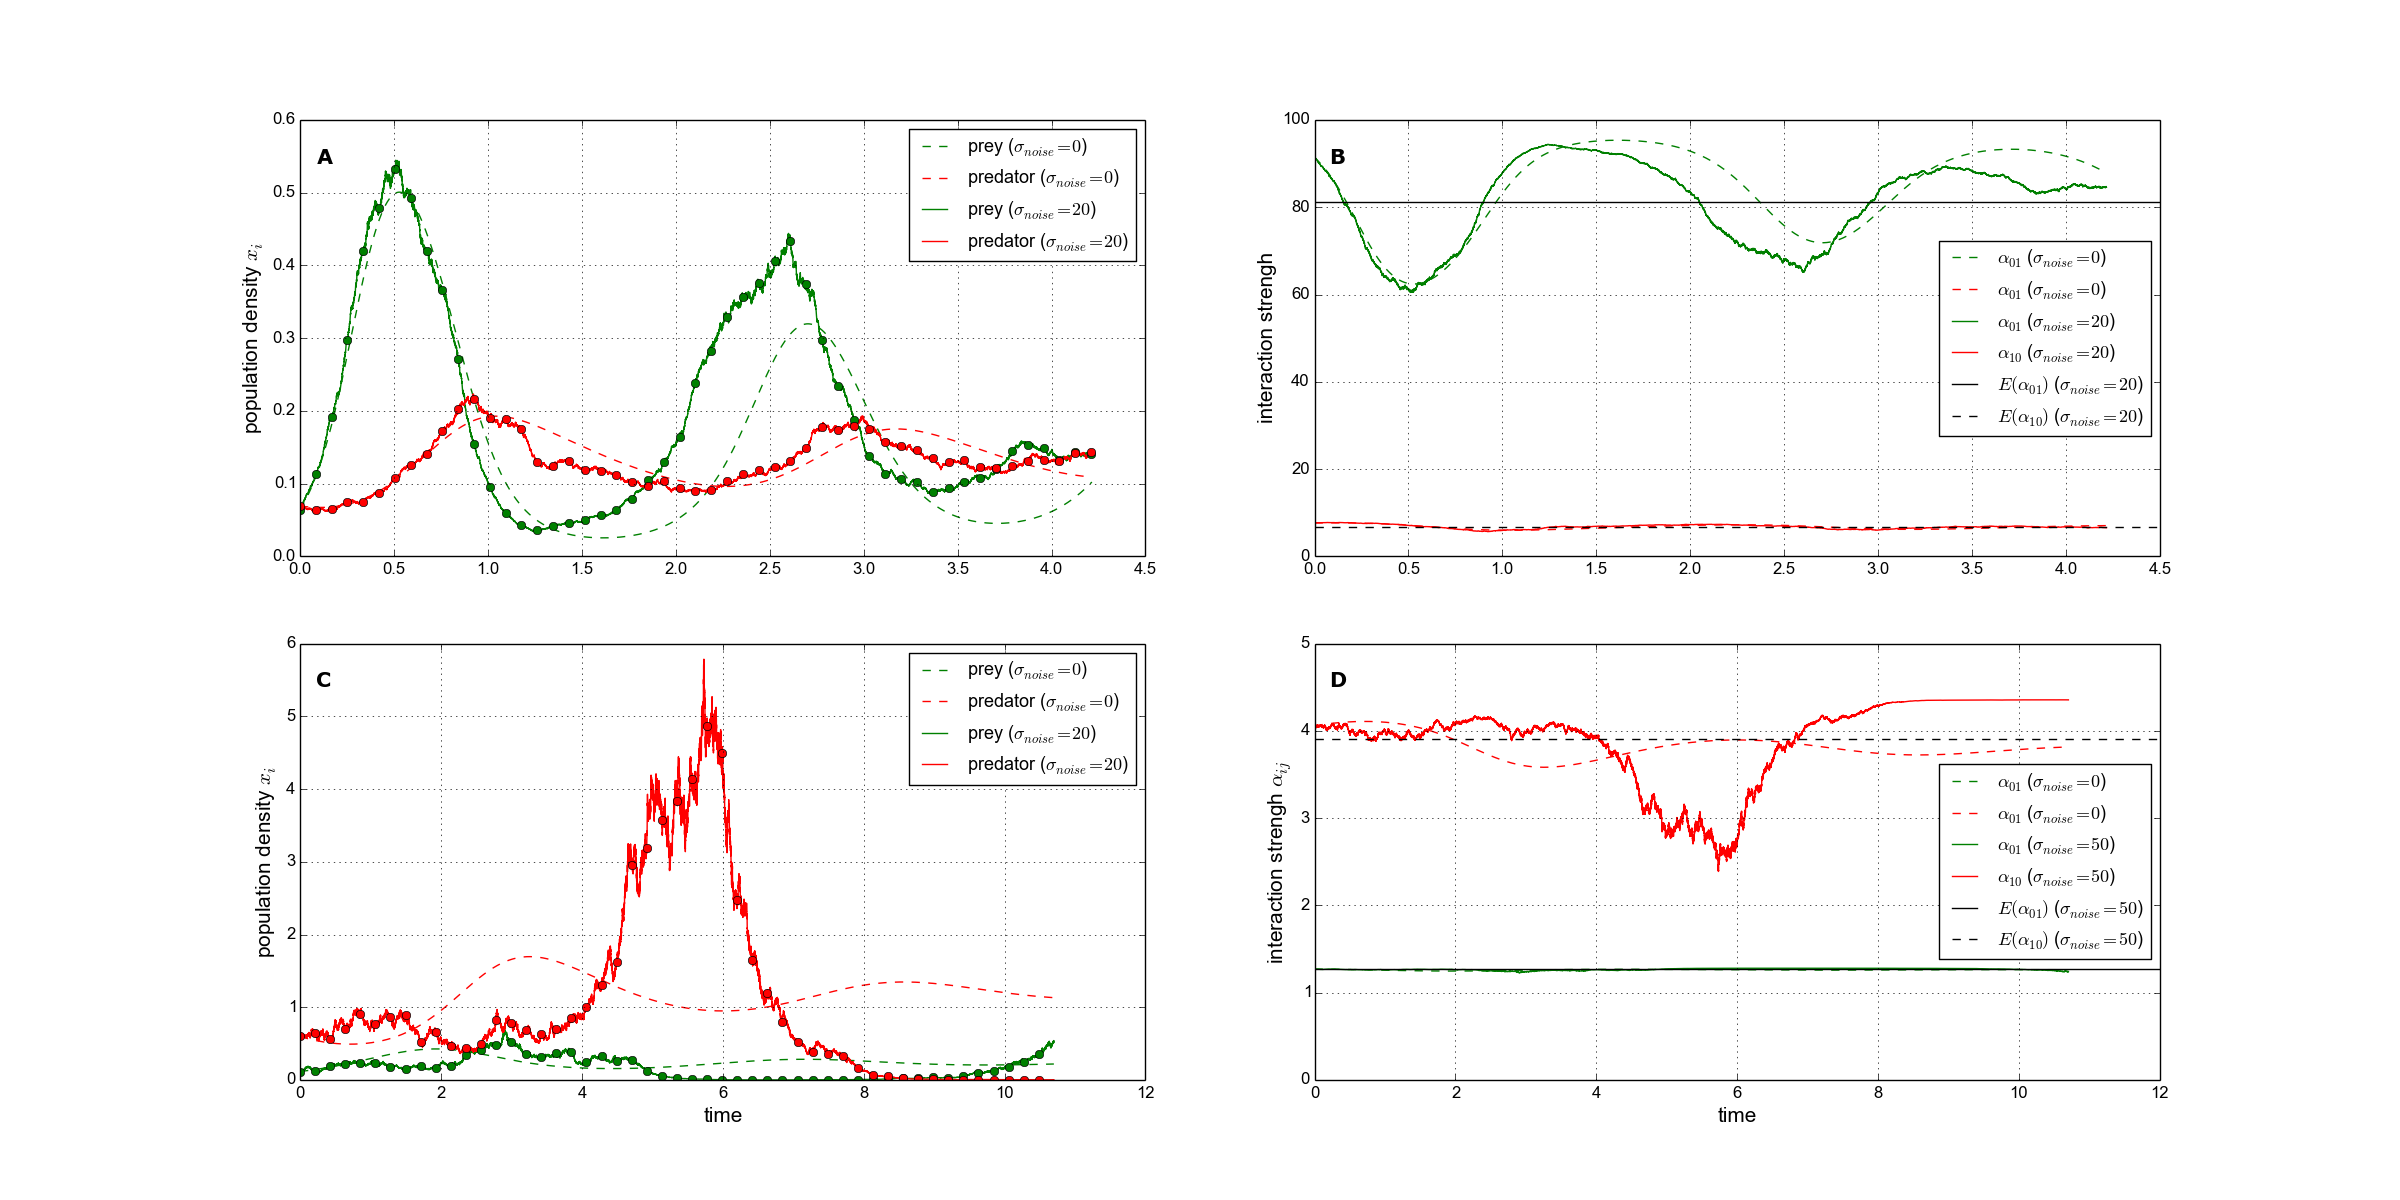
\includegraphics[width=\linewidth]{{{figures/example_dynamics_HII_pID_7_and_0}}}
		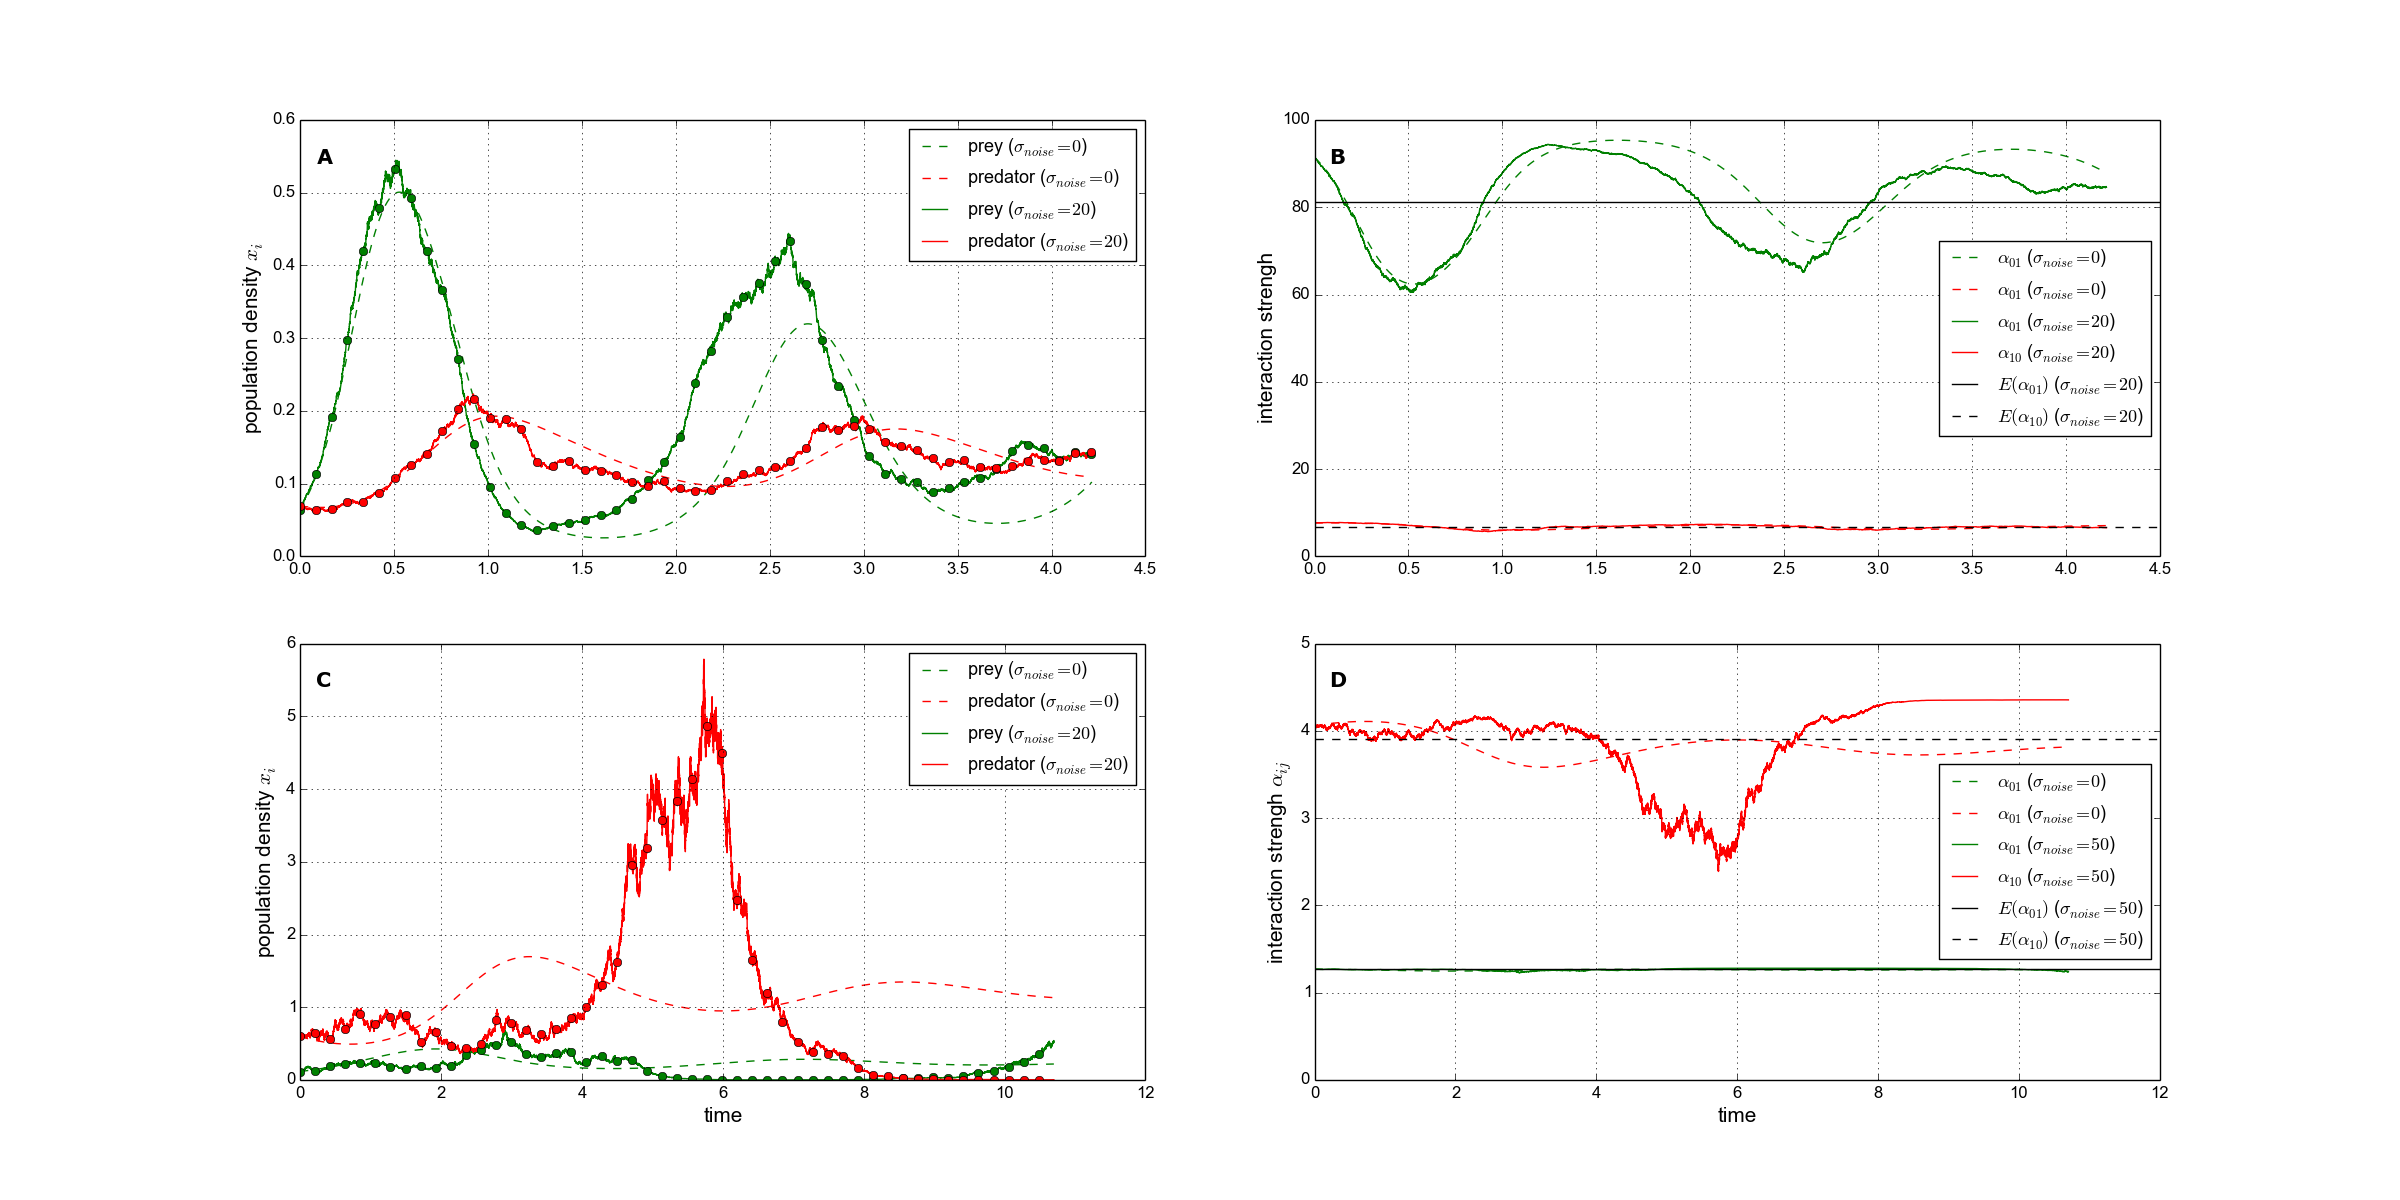
\includegraphics[width=\textwidth]{{{figures/example_dynamics_HII_pID_7_and_0}}}
        \caption{Example HOlling II dynamics.}\label{fig:ex_dynamics_holling}
        %% Note: this figure generated by Documents/IM_vs_HL_heatmap/plot_sum_maps.py
\end{sidewaysfigure}
\clearpage
%}

\section{Results}
\label{sec:results}

% some of this description goes above - for example some need explaining before previous section(examples)
In this sections we characterise the numerical performance of the method, described in section \ref{sec:timme}, for estimating the strength of interactions between species. The method is tested on the dynamics of two different ODE systems: a Lotka-Volterra (LV) and a Holling type II (HII) system. In the first case it is simply a test of a model fitting procedure. This is because the method works by fitting a generalised Lotka-Volterra (GLV) model to the dynamics, and he LV systems can be expressed as a GLV systems. Therefore we are simply simulating using one model, and then testing a method of estimating the model parameters form the simulated dynamics. We test the effects of noise and sampling frequency. In the second case, the HII system cannot be expressed as a GLV system. Therefore the GLV model that we fit can only approximate the dynamics and we cannot make a direct comparison between the parameters of the simulation model and the GLV model used for estimation. In this case we comapre to the mean interaction strengths (see section \ref{sec:res_hii}.


\subsection{Linear model}
\label{sec:res_glv}

Initially we run repeated simulations of the LV model using a single parameter set. We investigate how the numerical estimates of the model parameters respond to two variables: the level of noise in the simulations; and the number of samples used for estimation. Other variables are held constant using the simulation procedure described in section \ref{sec:simulation_method}. We then generalise these results by looking at the relative error in the estimates, for repeated simulations using an ensemble of 100 selected parameter sets (as described in section \ref{sec:simulation_method}).

\paragraph*{Single parameter set.}

Here we can make direct comparison between model parameters. The GLV model for two species has six parameters: $r_0,r_1,J_{00},J_{01},J_{10},J_{11}$. These correspond respectively to the following constant values of the LV system used for simulations: $A,-1,-A,-B,C,0$ (see equation \ref{eq:WHEREIS}). In general we find that the numerical estimates perform well at low noise intensities and poorly at high noise intensities. This is illustrated in figures \ref{fig:sp_v_n_100} and \ref{fig:sp_v_n_10000}. We also find that the estimates improve with the number of samples used, up to a point. Beyond this point the use of more samples does little to improve to estimates, and in some cases makes them worse. This behaviour is illustrated in figures \ref{fig:sp_v_ns_10} and \ref{fig:sp_v_ns_50}. These patterns were found to hold across all parameter sets investiagted, but are only shown using a single parameter set here for clarity.

In panel \textbf{A} of figures \ref{fig:sp_v_n_100} and \ref{fig:sp_v_n_10000} we see that the mean value of the estimates approaches the true value for low noise and, in panel \textbf{B} that the variance in the estimates approaches zero. This tells us that the method consistently gives a good fit of the GLV to the dynamics of the LV system, even when only 100 sample points are used (figure \ref{fig:sp_v_n_100}). As the noise intesitiy is increased the mean values of the estimates deviate from the true values, and the standard deviation in the estimates increases. Comparing the two figures we see that the response to noise is very similar whether 100 or 10,000 samples are used. A notable exception to this is a spike in the variance in panel \textbf{B} of figure. However this appears to be a single statistically anomolous result and not part of the trend. Panel \textbf{C} of both figures shows that the error function, which is minimised by the estimation method, increases with noise for both species. This cannot be directly compared between the two plots because of the different number of samples used. However it indicates that in both cases (100 and 10,000 samples) the quality of the fit is high in the deterministic case, and decreases with noise. 

\begin{figure}[h]
\centering 
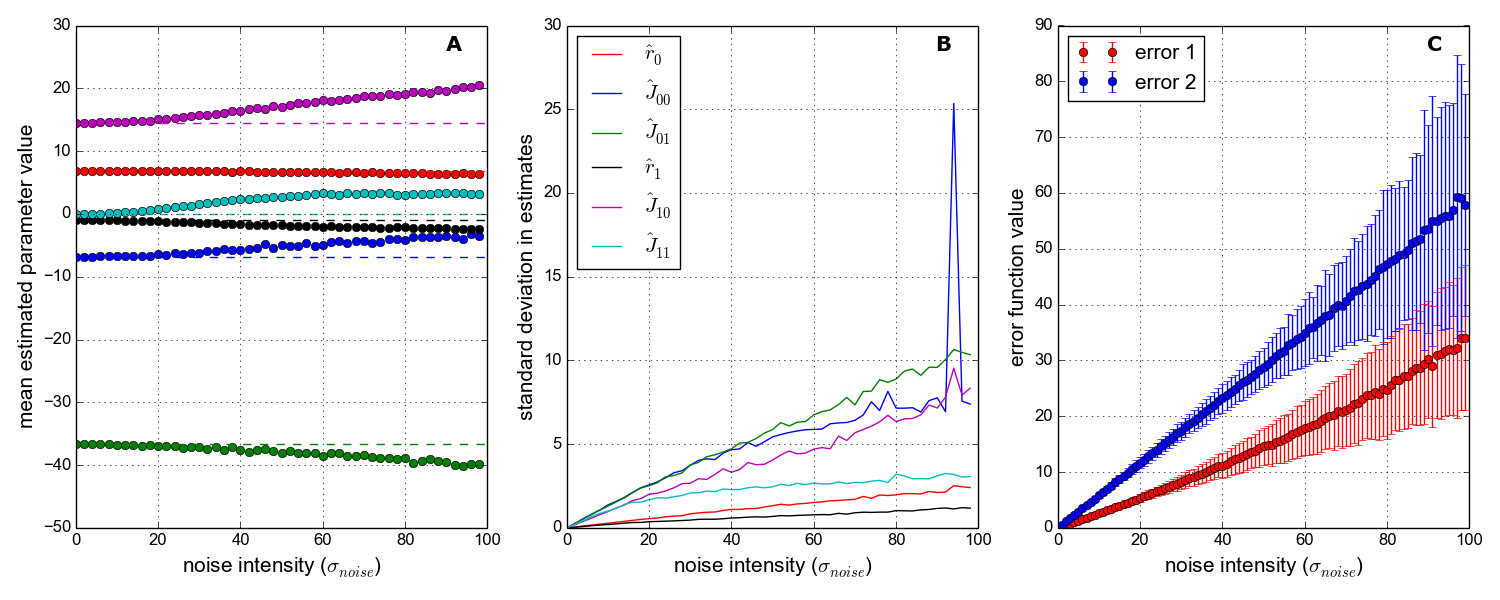
\includegraphics[width=\textwidth]{{{figures/single_params_v_noise_pID_0_nsamples_100}}}
\caption{Effect of noise on numerical estimates. Here the method uses 100 samples from simulated dynamics. All simulations run using the LV model with a single parameter set. The noise intensity varies between 0 (deterministic) and 100. See section \ref{sec:method_examples} for an intuition of how noisy this is. 1000 repeat smulations run at each noise level. \textbf{Panel A}: Mean estimated parameter values (each dot representing mean over 1000 repeats). The `true' paramter values of the simulation model are shown by dashed lines. \textbf{Panel B:} Standard deviation in estimates. \textbf{Panel C:} Value of the error functions used in the estimation method, one for each species. The dots show the mean error, and the bars show $\pm$ one standard deviation.}
\label{fig:sp_v_n_100}
\end{figure}

\begin{figure}[h]
\centering 
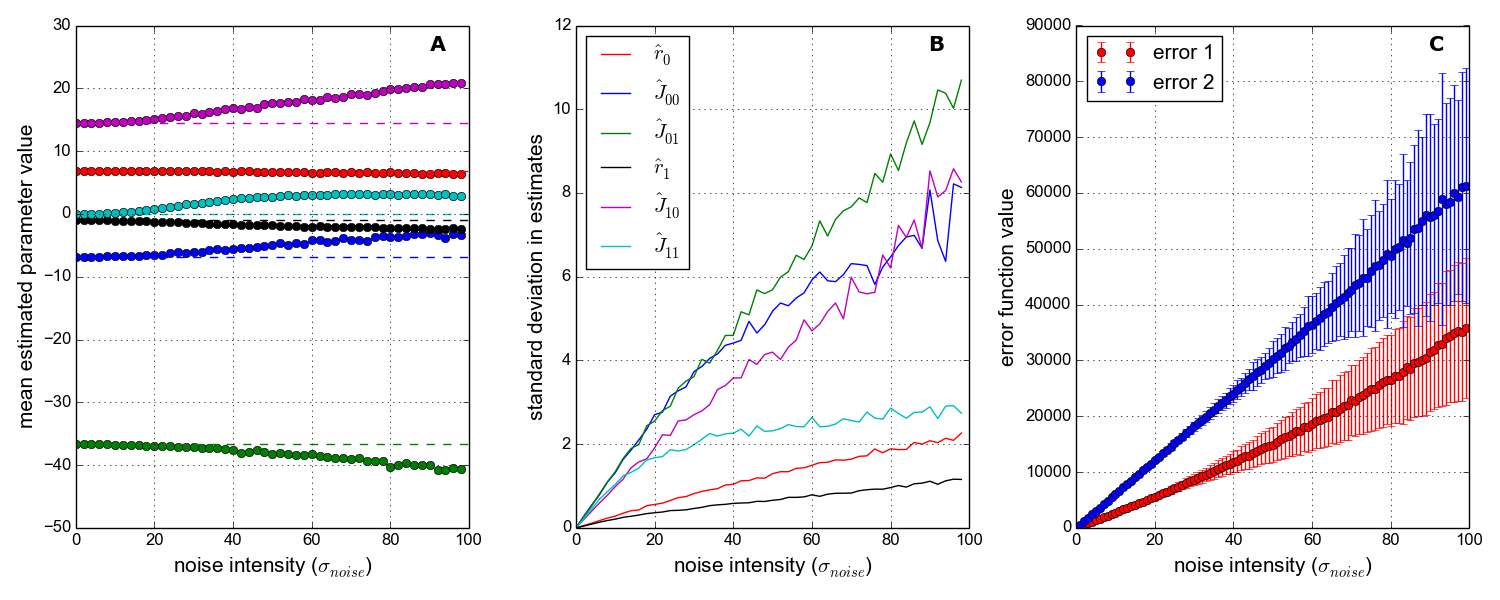
\includegraphics[width=\textwidth]{{{figures/single_params_v_noise_pID_0_nsamples_10000}}}
\caption{Exactly as in figure \ref{fig:sp_v_n_100} but using 10,000 samples from the simulated dynamics.} 
\label{fig:sp_v_n_10000}
\end{figure}

We now look at how the estimates respond to the number of samples used, in the cases of low and high noise intensity. Figure \ref{fig:sp_v_ns_10} shows the low noise case, with $\sigma_{noise}=10$. In panel \textbf{A} we see that the mean value of the estimates quickly converges to close to the true parameter values, as the number of samples increases. Panel \textbf{B} shows that the standard deviation in the estimates quickly becomes small, but non-zero. Above about 32 samples there is no visible improvement in the estimates, as measured by the mean or standard deviation. In figure \ref{fig:sp_v_ns_50} we see the effect of a higher noise intensity. Here we have $\sigma_{noise}=50$. Panel \textbf{A} shows that the estimates do not converge on the true parameter values, even for large numbers of samples. Also the standard deviation in the estimates, shown in panel \textbf{B}, is higher than in the low noise case. Again we find that there is little, if any, improvement in the estimates beyond about 32 samples. 
%% also general ruel: intirnsic growth parameters are better matched..

\begin{figure}[h]
\centering 
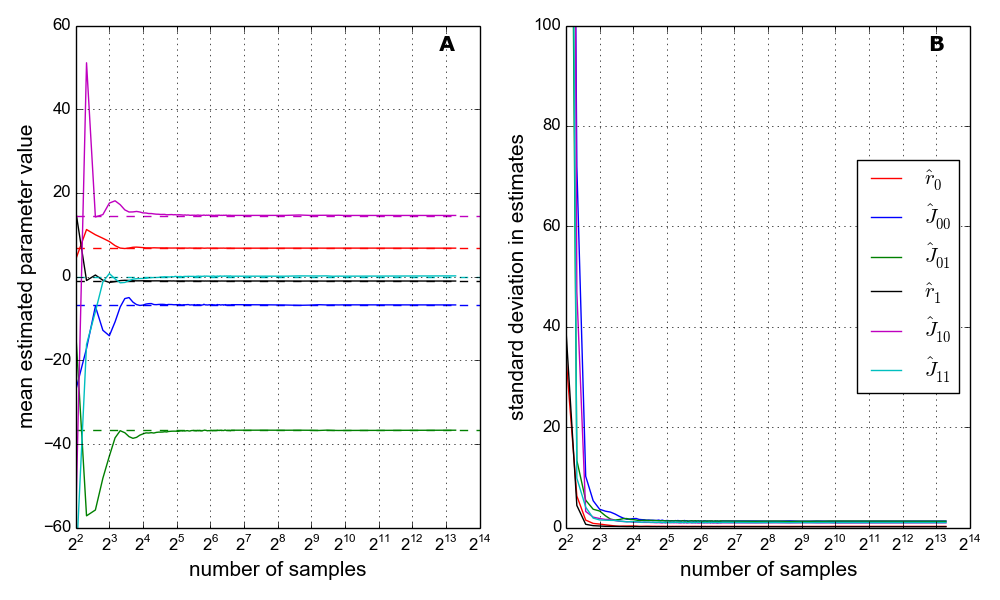
\includegraphics[width=0.67\textwidth]{{{figures/single_params_v_nsamples_pID_0_noise_10.000000}}}
\caption{Effect of the number of samples on numerical estimates. All simulations run using the LV model with a single parameter set. The noise intensity $\sigma_{noise}=10$. Number of samples ranges from 4 to 10,000. Samples drawn from  simulated dynamics at equal intervals. 1000 repeat smulations for each number of samples. \textbf{Panel A}: Solid lines show mean estimated parameter values. Dashed lines show the `true' paramter values of the simulation model. \textbf{Panel B:} Standard deviation in estimates.}
\label{fig:sp_v_ns_10}
\end{figure}

\begin{figure}[h]
\centering 
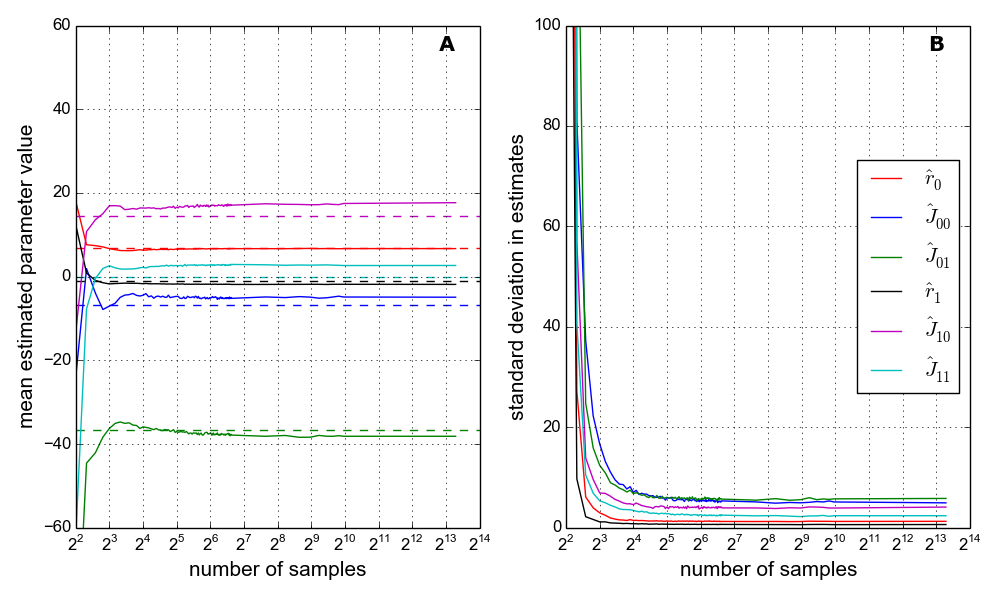
\includegraphics[width=0.67\textwidth]{{{figures/single_params_v_nsamples_pID_0_noise_50.000000}}}
\caption{Exactly as in figure \ref{fig:sp_v_ns_10} but with noise intesity $\sigma_{noise}=50$.} 
\label{fig:sp_v_ns_50}
\end{figure}

\paragraph*{Ensemble of parameter sets.}

Run 10 repeats for each of 100 parameter sets. In general the trends described above hold across the ensemble..

\begin{figure}[h]
\centering 
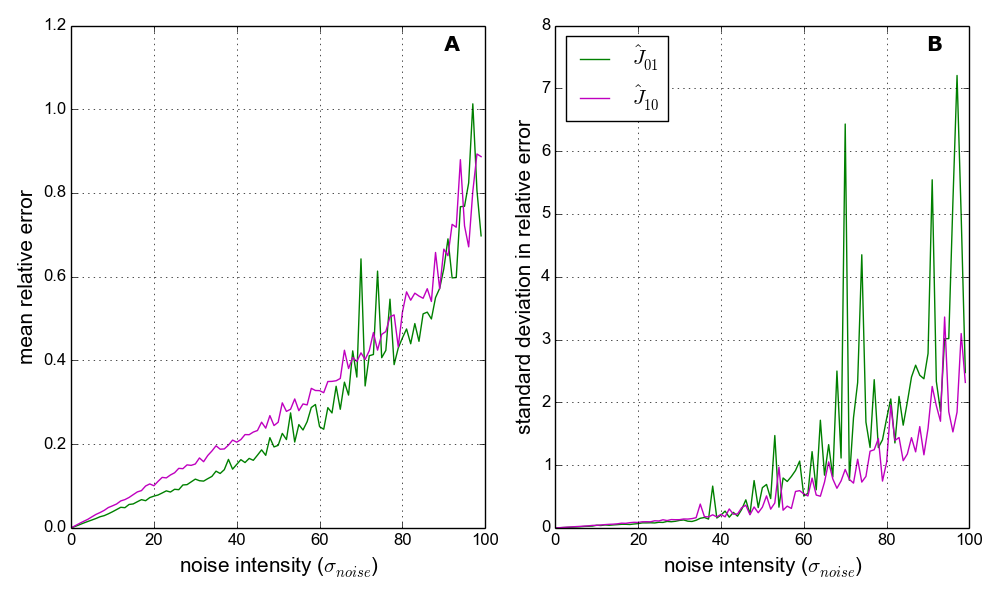
\includegraphics[width=0.67\textwidth]{{{figures/ensemble_params_vs_noise_nsamples_1000}}}
\caption{Nonsense. 1000 samples used.} 
\label{fig:ep_v_n}
\end{figure}

\begin{figure}[h]
\centering 
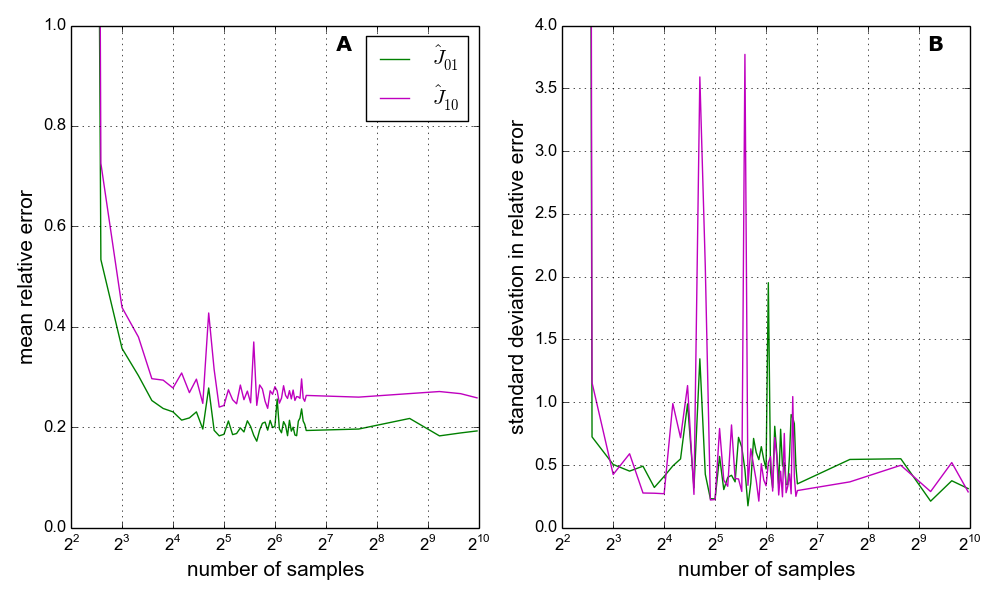
\includegraphics[width=0.67\textwidth]{{{figures/ensemble_params_vs_nsamples_noise_50.000000.IS}}}
\caption{Nonsense. Noise is 50.} 
\label{fig:ep_v_ns}
\end{figure}




\subsection{Holling model}
\label{sec:res_hii}

\begin{figure}[h]
\centering 
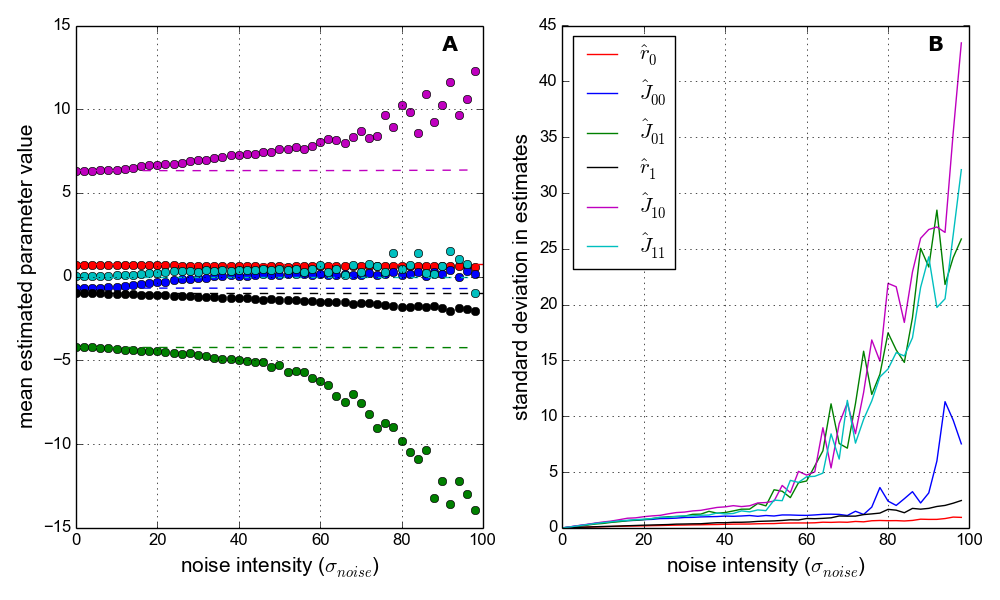
\includegraphics[width=0.67\textwidth]{{{figures/single_params_v_noise_pID_87_nsamples_10000.HII}}}
\caption{Nsamples is 10,000.} 
\label{fig:hii_sp_v_n}
\end{figure}

\begin{figure}[h]
\centering 
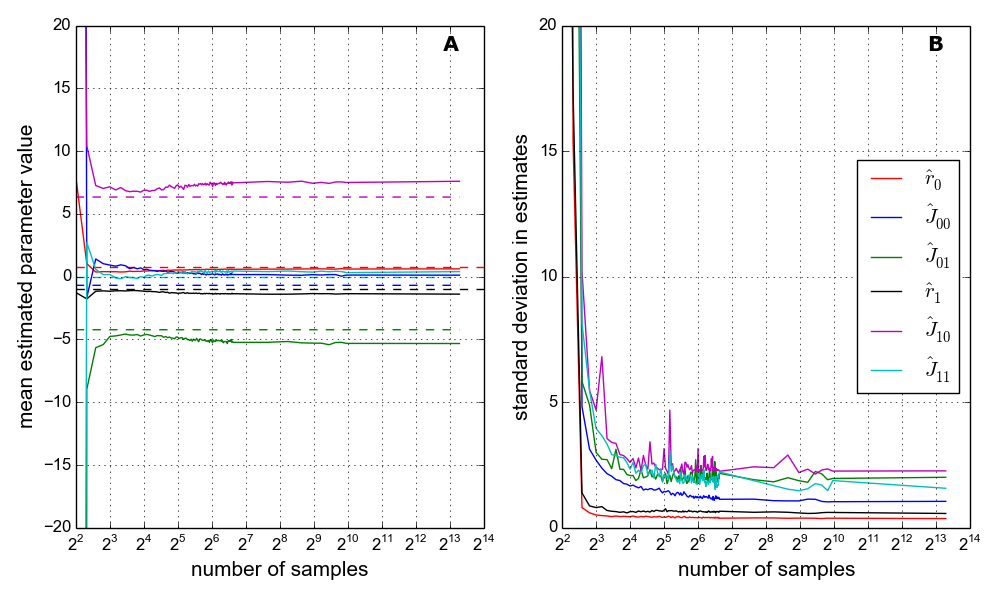
\includegraphics[width=0.67\textwidth]{{{figures/single_params_v_nsamples_pID_87_noise_50.000000.HII}}}
\caption{Noise is 50.} 
\label{fig:hii_sp_v_ns}
\end{figure}

\begin{figure}[h]
\centering 
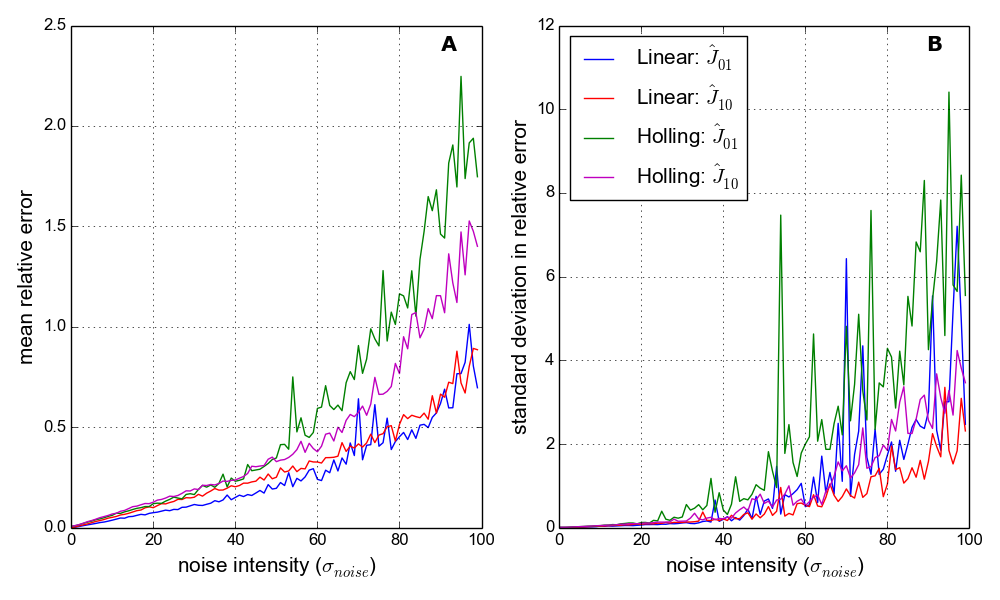
\includegraphics[width=0.67\textwidth]{{{figures/ensemble_params_vs_noise_nsamples_1000.B}}}
\caption{Noise is 50.} 
\label{fig:hii_ep_v_ns}
\end{figure}

\begin{figure}[h]
\centering 
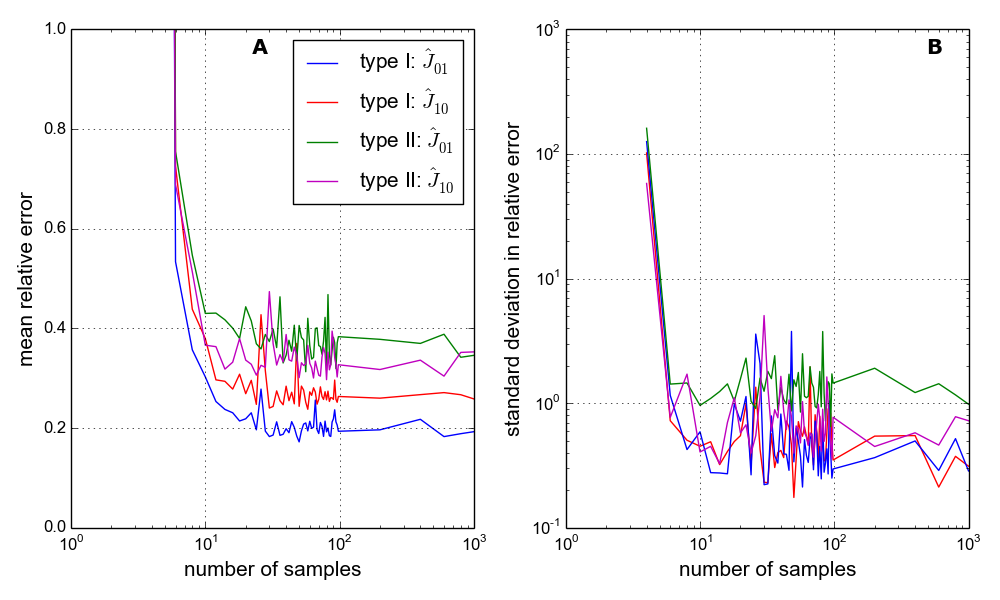
\includegraphics[width=0.67\textwidth]{{{figures/ensemble_params_vs_nsamples_noise_50.000000.B.IS}}}
\caption{Noise is 50.} 
\label{fig:hii_ep_v_ns}
\end{figure}


\subsection{Range sampling}
\label{sec:res_range_sampling}

%% Discussion of these results first??

% > only very few samples needed really!

\section{TEMP : other results}

This section shows some plots which I was not planning to put into the thesis but are worth discussing..

\begin{figure}[h]
\centering 
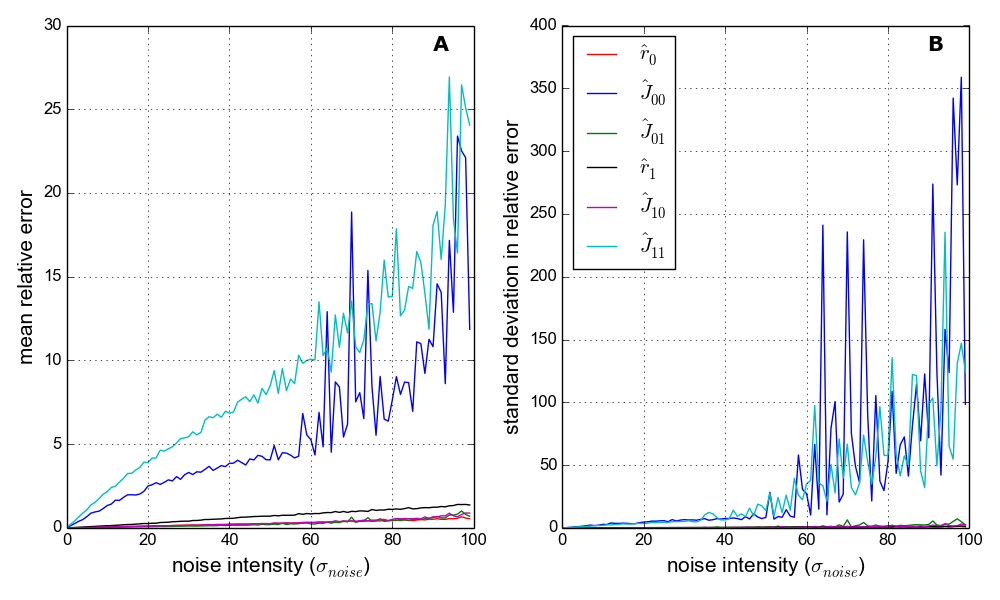
\includegraphics[width=0.67\textwidth]{{{figures/ensemble_params_vs_noise_nsamples_1000.ALL}}}
\caption{Nonsense. 1000 samples used.} 
\label{fig:ep_v_n}
\end{figure}

\begin{figure}[h]
\centering 
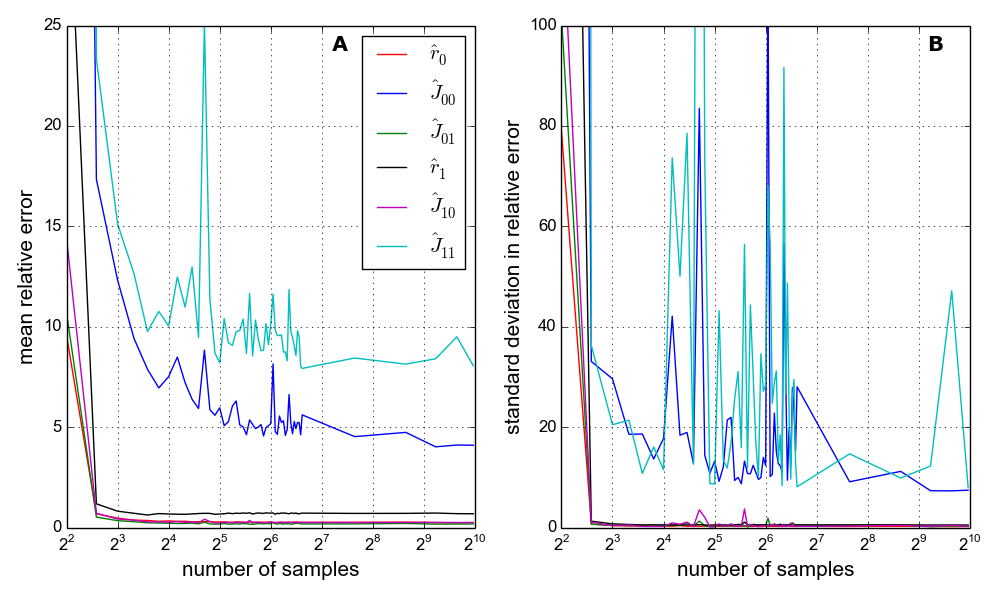
\includegraphics[width=0.67\textwidth]{{{figures/ensemble_params_vs_nsamples_noise_50.000000.ALL}}}
\caption{Nonsense. Noise is 50.} 
\label{fig:ep_v_ns}
\end{figure}

\section{Application to IBM (optional)}
\label{sec:ibm}

In this section we apply the methodology for inferring species interactions to the IBM simulations. In the previous section we have seen that the method works well when fitting the GLV to two species predator-prey dynamics simulated with ODE models. In the case that the dynamics is governed by the Lotkva-Volterra equations, and in the absence of noise, fitting the GLV model produces true estimates of the underlying parameters which include the inter-specific interaction strengths. The estimates require relatively few samples in order to achieve high accuracy, and which converge on the true parameter values as the sampling intensity increases. However as noise is added to the simulations the accuracy of the estimates decreases. In particular we found that, in the presence of noise, the estimates do not converge on the true parameter values - that is, noise introduces systematic error in to the estimates. In the case that the dynamics are governed by the Holling II model matters are complicated - but in general we find that the GLV can approximately capture the strength of species interactions (and also the dynamics?), provided there is not too much noise, and the FR is not too non-linear\footnote{This is all need to be demonstrated - WORK TO DO!}.

Can the IBM dynamics by approximated by the GLV model? The hypothesis is that is can. Argue this..and refer to previous mention of LV type dynamics. Refer forward to testing linearity of FR. Exponential growth and decay, linear FR. However there are certain problem/factors that may hinder this approach/represent a departure from GLV dynamics...Noise, spatial effects, bioenergetic model - time delay? Immigration (one component of noise).

The issue of noise is important since, as we have shown in chapter REF, there is a strong stochastic component to the IBM simulations. 

Modelling individuals, not biomass or energy. Is this problematic? Set herb-frac to 1. Other issues?

\subsection{Testing functional response (and intrinsic growth functions)}

Here we demonstrate the linearity of the predator functional response for animal predators in the second and third trophic levels (using 2sp and 3sp chain) - demonstrate that there is a slight difference. But basically linear. Other issues that may arise - high noise and low abundances create error. 

We also conduct an experiment to test the intrinsic growth and death rates of plant and animal species - by setting herb-frac=0.0. Demonstrate they are well approximated by exponential. In the absence of immigration. 

Carrying capacity: is there evidence for density dependent birth/death? - use this fact in later analysis. Also discuss that the carrying capacity will vary with the number of species, not just a single species thing (non-pairwise interactions in competition for space - argghh!)

\subsection{2 Species IBM model}

IMPORTANT: carrying capacity depends on other species...introduce a new term into the model and test it?

Define the model and what the inferred parameters represent:

\begin{itemize}
	\item $J_{01}$: per-capita of rate consumption of the prey
	\item $J_{10}$: per-capita of rate reproduction of predator, due to consumption of prey. Not as well defined. But only source of predator births? Numerical response! (get REF)
	
	\item $J_{00}$: intra-specific regulation of prey growth - see carrying capacity experiment.
	
	\item $J_{11}$: intra-specific regulation of predator mortality? Check this. Expect zero? Or expect high number of predator means more reproduction because easier to find partner, therefore reduce mortality? Or increase birth rate. Not clear. Again SEE EXPERIMENT. 
	
	\item $r_0$: prey intrinsic growth rate. Estimate from exp?
	
	\item $r_1$: predator intrinsic mortality rate. Estimate from exp?
\end{itemize}

So we know what values to expect, or at least the signs. We can evaluate the model fit by comparing the values of these estimates with birth/death rates from the simulations. Although not totally fair. We can also simulate GLV with the inferred parameters - does it match. Is the equilibrium the same? And check the error function of the fit. We show all this in the results section below.

\paragraph*{Dynamics of the model} we two species is a new thing. Here we show that with the default parameters we get relaxation-type oscillations. This is interesting, we try fitting to these in the two species case. But they become problematic for larger number of species. Argue why. Therefore we increase the reproduction rate (refer to previous chapter), which creates more WORD dynamics. We also fit to these. 

PLOT: DYNAMICS UNDER IR, RR AND HL.

Also show dependence on immigration (show that it is low and what happens if it is high), concede that this is a limitation. 

\subsection{Extend methodology (3, 4 and 5 species)}

MULTI-SPECIES DENSITY DEPENDENCE?!

This does not require much since we presented a general framework previously. 

Show 3 species dynamics with the two different RR. Conclude which is better. 

\subsection{Results}

\subsection{2 species}

Here we compare the results of two species. 

For a single IR we look at convergence of all 6 parameters (over the ensemble) - correct signs, correct magnitudes?

Maybe repeat for other IRs and HL.

We then show rate estimates as time series and introduce quality metric for this\footnote{Still not sure about this}.

Demonstrate the quality decreases with IR and HL (box plot?).
And how estimated parameters respond to the two HL scenarios (refer to previous findings). Hopefully support!



%% TOD DISCUSS RE IBM APPLICATION:

% > could introduce non-linearities to IS. E.g. hanlding time?
% > discuss application to larger system. Functional groupings...etc.
\section{Discussion}
\label{sec:discussion}

Points referenced in text above, make sure to discuss them!..

\begin{itemize}
	\item Discuss how this methodology could be used on empircal data...
	\item Limitations of ODE models (non-spatial, repsonse to debate on FR)
	\item Possibility of extending to more than two specie systems (if this is actually done then change ref in text above)
	\item discussion of other forms of FR (not H) - or disucssed already in inro?
	
	\item good GLV fit to LV even with 100 sample points - realistic?
	
	\item how good is the method of model fitting. Discuss more computationally expensive options (mentioned in section on Timme method)
	
	\item Spatial heterogeneity - we do not explore this here, but acknowledge that it represents are source of error. Gives example in extremis - 2 species only interacting on boundary. Also we know that there is some level of spatial aggregation, especially at low IR - possibly show one plot of this?
	
	\item Could introduce prey handling to IBM to create non-linear FR.
	
	\item Our method could be used to pick out coupling to other variables e.g evironmental (temperature) if expressed in a certain way.
\end{itemize}
